\section{Hopfield モデル}


\cite{Hopfield1982-vu}で提案.始めは1と0の状態を取った.

Hopfieldモデルと呼ばれることが多いが,Amariの先駆的研究\cite{Amari1972-fq}を踏まえAmari-Hopfieldモデルと呼ばれることもある.

次のような連続時間線形モデルを考える.シナプス前活動を$\mathbf{x}\in \mathbb{R}^n$, 後活動を$\mathbf{y}\in \mathbb{R}^m$, 重み行列を$\mathbf{W}\in \mathbb{R}^{m\times n}$とする.


\begin{equation}
\frac{d\mathbf{y}}{dt}=-\mathbf{y}+\mathbf{W}\mathbf{x}+\mathbf{b}
\end{equation}


ここで$\dfrac{\partial\mathcal{L}}{\partial\mathbf{y}}\triangleq-\dfrac{d\mathbf{y}}{dt}$となるような$\mathcal{L}\in \mathbb{R}$を仮定すると,


\begin{equation}
\mathcal{L}=\int \left(\mathbf{y}-\mathbf{W}\mathbf{x}-\mathbf{b}\right)\ d\mathbf{y}=\frac{1}{2}\|\mathbf{y}\|^2-\mathbf{y}^\top \mathbf{W}\mathbf{x}-\mathbf{y}^\top \mathbf{b}
\end{equation}


となる. これをさらに$\mathbf{W}$で微分すると,


\begin{equation}
\dfrac{\partial\mathcal{L}}{\partial\mathbf{W}}=-\mathbf{y}\mathbf{x}^\top\Rightarrow
\frac{d\mathbf{W}}{dt}=-\dfrac{\partial\mathcal{L}}{\partial\mathbf{W}}=\mathbf{y}\mathbf{x}^\top=(\text{post})\cdot (\text{pre})^\top
\end{equation}


となり,Hebb則が導出できる.
\subsection{モデルの定義}
モデルを定義する.
\lstinputlisting[language=julia]{./text/energy-based-model/hopfield-model/002.jl}
\lstinputlisting[language=julia]{./text/energy-based-model/hopfield-model/003.jl}
\lstinputlisting[language=julia]{./text/energy-based-model/hopfield-model/004.jl}
データセットの作成
\lstinputlisting[language=julia]{./text/energy-based-model/hopfield-model/006.jl}
\lstinputlisting[language=julia]{./text/energy-based-model/hopfield-model/007.jl}
\begin{figure}[ht]
	\centering
	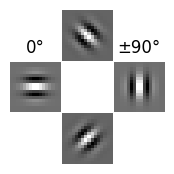
\includegraphics[scale=0.8, max width=\linewidth]{./fig/bayesian-brain/neural-sampling/cell007.png}
	\caption{cell007.png}
	\label{cell007.png}
\end{figure}
モデルの定義と訓練
\lstinputlisting[language=julia]{./text/energy-based-model/hopfield-model/009.jl}
\lstinputlisting[language=julia]{./text/energy-based-model/hopfield-model/010.jl}
\begin{figure}[ht]
	\centering
	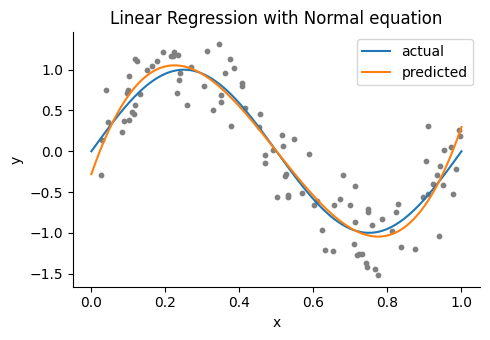
\includegraphics[scale=0.8, max width=\linewidth]{./fig/introduction/linear-regression/cell010.png}
	\caption{cell010.png}
	\label{cell010.png}
\end{figure}
画像の復元を行う.
エネルギー関数


\begin{equation}
E=-{\frac 12}\sum _{{i,j}}{w_{{ij}}{s_{i}}{s_{j}}}+\sum _{i}{\theta _{i}}{s_{i}}=-{\frac 12}\mathbf{s}^\top\mathbf{W}\mathbf{s}+\mathbf{\theta}^\top\mathbf{s}
\end{equation}


を最小化するように内部状態 $\mathbf{s}$ を更新.


\begin{equation}
\mathbf{s}\leftarrow \text{sign}\left(\mathbf{W}\mathbf{s}-\mathbf{\theta}\right)
\end{equation}
\lstinputlisting[language=julia]{./text/energy-based-model/hopfield-model/012.jl}
\lstinputlisting[language=julia]{./text/energy-based-model/hopfield-model/013.jl}
\lstinputlisting[language=julia]{./text/energy-based-model/hopfield-model/014.jl}
\begin{figure}[ht]
	\centering
	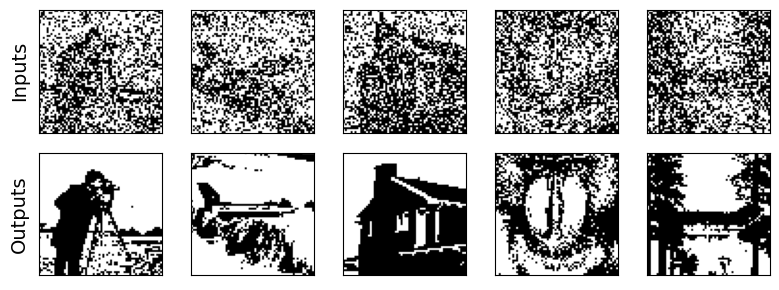
\includegraphics[scale=0.8, max width=\linewidth]{./fig/energy-based-model/hopfield-model/cell014.png}
	\caption{cell014.png}
	\label{cell014.png}
\end{figure}
\subsection{稠密連想記憶 (dense associative memory) モデル}
\textbf{\index{Dense Associative Memory (DAM)}} モデル (Modern Hopfield networksとも呼ばれる) .

\begin{itemize}
\item Krotov, Dmitry, and John J. Hopfield. 2016. “Dense Associative Memory for Pattern Recognition.” arXiv. arXiv. \url{http://arxiv.org/abs/1606.01164}.
\item Krotov, Dmitry, and John Hopfield. 2018. “Dense Associative Memory Is Robust to Adversarial Inputs.” Neural Computation 30 (12): 3151–67.
\item Krotov, Dmitry, and John J. Hopfield. 2019. “Unsupervised Learning by Competing Hidden Units.” Proceedings of the National Academy of Sciences of the United States of America 116 (16): 7723–31.
\end{itemize}


\begin{itemize}
\item Ramsauer, Hubert, Bernhard Schäfl, Johannes Lehner, Philipp Seidl, Michael Widrich, Thomas Adler, Lukas Gruber, et al. 2020. “Hopfield Networks Is All You Need.” arXiv. arXiv. \url{http://arxiv.org/abs/2008.02217}.
\end{itemize}

深層ニューラルネットワークへの応用.


\begin{itemize}
\item Krotov, Dmitry, and John J. Hopfield. 2020. “Large Associative Memory Problem in Neurobiology and Machine Learning.” \url{https://openreview.net/pdf?id=X4y_10OX-hX}
\end{itemize}

“Hopfield Networks Is All You Need.”の論文における非生理学的3ニューロン相互作用の緩和.
